\section{Female Education and Labor Force Participation in India}

Female educational attainment has increased substantially over time.
Figure \ref{fig:education_over_time} shows the distribution of schooling by birth 
cohort for urban and rural women, 
twenty years or older, whether married or not, based on the four rounds of the NFHS.
The education groups are no education, one to seven years, and eight to eleven years,
and twelve years and above.

\begin{figure}[htpb]
\centering
\subfloat[Rural]{
    \begin{minipage}{0.49\textwidth}
        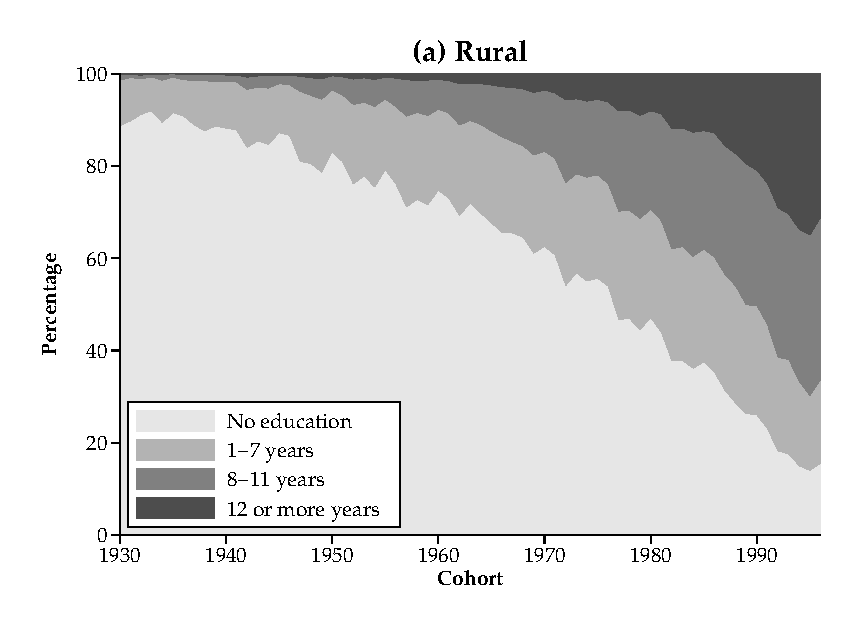
\includegraphics[width=\textwidth]{educ_over_time_rural}
    \end{minipage}
} 
\subfloat[Urban]{
    \begin{minipage}{0.49\textwidth}
        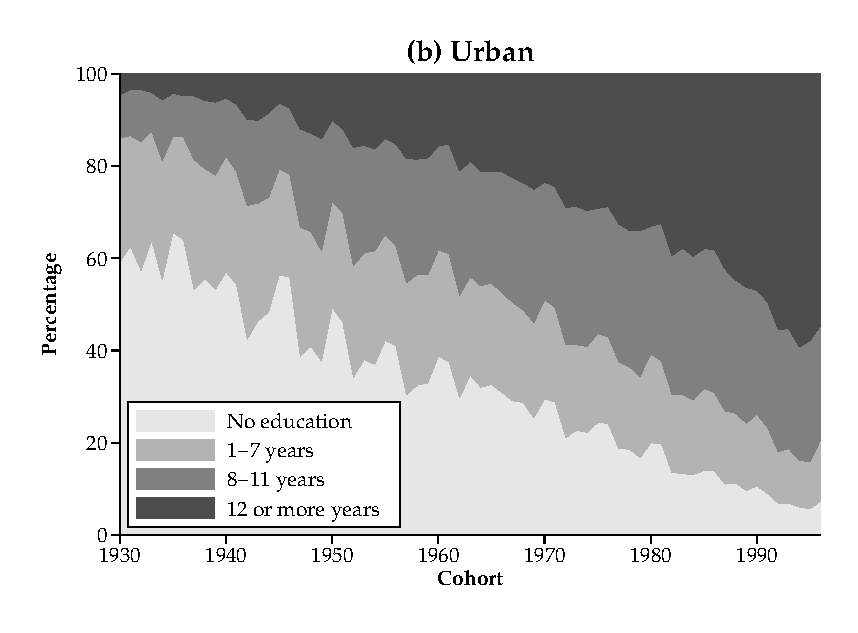
\includegraphics[width=\textwidth]{educ_over_time_urban} 
    \end{minipage}
}
\caption{Distribution of education by cohort for women twenty years or older at survey}
\label{fig:education_over_time}
\end{figure}


For rural areas, the percentage of women with no education has gone from around 90 percent
for the 1930s cohorts to less than 20 percent for the 1990s cohorts. 
The proportion of women with one to seven years of education has remained remarkably
constant at around ten percent.
The difference is made up by the women with eight or more years of education, who have
gone from almost zero for the 1930 cohort to more than sixty percent for the 1990s cohorts,
with about half in the eight to eleven years group and 
the other half in the twelve years or more group.

Female education is higher in urban areas than in rural areas.
Around sixty percent of urban women born in the 1930s had no education, 25 percent had
between one and seven years, about 10 had eight or more years of education, and only
five percent has twelve years or more.
The proportions with no education and one to seven years have both declined to just below 
ten percent for the latest cohort.
Although the proportion of women with eight to eleven years of education has increased
to about twenty, most of the increase in urban female education has come from the 
twelve plus group, which now account for more than half of all urban women.

Even as the level of female education has increased, the female labor force participation 
in both urban and rural areas has stagnated or decreased
\citep{Klasen2015,Afridi2018,Bhargava2018,Chatterjee2018,Bhargava2019}.
A decline in female labor force participation at the beginning of development is
consistent with the hypothesis of a U-shaped labor force participation as a country
develops \citep{Goldin1994}.
India's female labor force participation is, however, lower than most other
countries and more in line with countries in the Middle East and North Africa, and
does not yet show any signs of increasing
\citep{Klasen2015,Chatterjee2018}.

Theory predicts that increasing women's wages leads to higher labor force participation, 
while both a higher male income and stronger social restrictions on working, possibly in 
specific industries or jobs, reduce female labor supply \citep{Goldin1994}.
India's economy has grown substantially since the mid-seventies, with
an average annual growth rate of about 5.5 percent from 1978 to 2004 \citet{Bosworth2008}.
As a result, real wages for both men and women have almost doubled between 1987 and 2011 
\citep{Klasen2015}.
Despite the increases in wages and the higher female education, the mean male wage is
still close to 70 percent higher than the mean female wage \citep{Bhargava2018}.
Furthermore, the development in women's wages is not uniform across education 
levels \citep{Klasen2015,Bhargava2018}.
The real wages for women with middle school education or below have converged. 
For women with secondary education, the change over time depends on the sample used,
with some showing a substantial decline and others a modest increase.
Women with more than secondary education experienced an increased in their real 
wages, especially in cities.

After controlling for household characteristics and husband income, there is
still a U-shaped relationship between female education and labor supply with the
lowest labor force participation for women with secondary education \citep{Chatterjee2018}.
There are two possible explanations for this effect, both directly related to the strong
pro-male bias in India.
First, it becomes less socially acceptable for women to work in manual labor as their
education increases, and women are still mostly excluded from white-collar
employment despite robust economic growth \citep{Klasen2015,Chatterjee2018}.
Second, with increasing education, women's productivity at home also increases, especially
in the production of offspring human capital.
With relatively more boys born because of increased access to sex-selective 
abortions and an increasing male income, demand for better-educated women can 
increase, even if they do not participate in the labor market \citep{Behrman1999}.

Figure \ref{fig:work_by_survey} shows the percent of married women who are 
currently working at the time of the survey by age group and education level.
No other labor force participation question is consistently available across all 
four surveys. 
Because the question refers to currently working, the percentages will be lower 
than what other studies have found. 
Furthermore, since the question is asked only of married women, the overall female labor 
force participation might have developed differently, especially since many young, 
unmarried women have begun working in, for example, the business process 
outsourcing industry, which, in turn, has increased girls' schooling investments
\citep{Jensen2012}.

\begin{figure}[!htpb]
\centering
\rotatebox[origin=c]{90}{\small{40 Years or Older}}
\subfloat[Rural]{
    \begin{minipage}{0.45\textwidth}
        \includegraphics[width=\textwidth]{currently_working_rural_40}
    \end{minipage}
} 
\subfloat[Urban]{
    \begin{minipage}{0.45\textwidth}
        \includegraphics[width=\textwidth]{currently_working_urban_40} 
    \end{minipage}
}
\\
\rotatebox[origin=c]{90}{\small{30 to 39 Years Old}}
\subfloat[Rural]{
    \begin{minipage}{0.45\textwidth}
        \includegraphics[width=\textwidth]{currently_working_rural_30}
    \end{minipage}
} 
\subfloat[Urban]{
    \begin{minipage}{0.45\textwidth}
        \includegraphics[width=\textwidth]{currently_working_urban_30} 
    \end{minipage}
}
\\
\rotatebox[origin=c]{90}{\small{20 to 29 Years Old}}
\subfloat[Rural]{
    \begin{minipage}{0.45\textwidth}
        \includegraphics[width=\textwidth]{currently_working_rural_20}
    \end{minipage}
} 
\subfloat[Urban]{
    \begin{minipage}{0.45\textwidth}
        \includegraphics[width=\textwidth]{currently_working_urban_20} 
    \end{minipage}
}
\caption{Percentage of married women who were working at the time of the 
survey by age group and area of residence}
\label{fig:work_by_survey}
\end{figure}


The U-shaped relationship between education and working holds in most cases with 
the highest percent working for women with either no education or with twelve or 
more years and the lowest for women with eight to eleven years of education.
Women are more likely to report working if they live in rural than urban areas 
and the older they are.
Comparing 1992 and 2015, the percent of women who currently work has either 
remained roughly the same or decreased.
The cases were the numbers were higher in 1999 and 2006 than in 1992 or 2015 
are mostly based on small samples, such as rural women with twelve or more 
years of education in rural areas.

Almost all of the urban women who work receive either cash or a combination of 
cash and in-kind for their work (see Appendix Figure \ref{fig:work_cash_by_survey}). 
Rural women have become more likely to receive cash for their labor over time, 
and the better educated, the more likely they are to receive cash.

Despite this, women across all groups have become substantially more likely to 
work for a family member rather than for themselves or somebody else
(see Appendix Figure \ref{fig:work_family_by_survey}).
Hence, the lower likelihood of working stems mostly from women retracting from 
the general labor market and self-employment.

The increases in female educational attainment imply that access to education 
has expanded beyond the higher castes. 
However, ``Sanskritization'' implies that as lower castes females gain access to 
education and their husbands' income increases, the women adopt higher caste 
norms such as stronger son preference and a retraction from the formal labor 
market \citep{Srinivas1956,Chen1995,Abraham2013,Chatterjee2018}. 
``Sanskritization'' may also lead to an increased aversion to daughters, rather 
than just an increased preference for sons, which, in turn, lowers desired 
fertility \citep{Borooah2004}.

Hence, with substantial increases in husband income and a declining female labor force 
participation, I expect a push toward longer birth spacing over time, independent
of education levels, based on the income effects and the effects of spacing
on child outcomes in the theories above.
The declining percentage of women working suggests that the opportunity cost
effects with increasing education will not be strong enough to shorten the
birth spacing.

As desired fertility decreases with increasing education, I, furthermore, expect 
birth spacing to increase the most among the best-educated because of their 
use of sex selection and because of "Sanskritization" the changing composition 
of women in the better-educated group does not substantially change this 
group's use of sex selection.
Working in the opposite direction is that women with more education can space
their children closer together without substantially increasing child mortality risk.


